\subsubsection{Estensione A: Prezzo della Controproposta Mancante}

Durante la compilazione della controproposta, l’agente potrebbe tentare di inviare il modulo senza aver specificato il prezzo proposto.  
Per prevenire errori di input e garantire l’integrità dei dati inviati al sistema, viene implementato un controllo di validazione lato client e lato server.

\subsubsection{Gestione del Messaggio di Errore}
Nel momento in cui l’agente clicca su \textbf{“Invia controproposta”} con il campo del prezzo vuoto, il sistema mostra un messaggio di errore direttamente sotto l’input della controproposta.  
Questo messaggio informa chiaramente l’utente dell’obbligo di compilare il campo prima di procedere.

L’interfaccia rimane attiva e consente all’agente di inserire il valore corretto e riprovare l’invio, tornando così al flusso principale dello scenario (Step 6).  

Questa scelta progettuale segue il principio della \textbf{visibilità dello stato del sistema} \cite{nielsen1995}, migliorando la chiarezza e riducendo la frustrazione dell’utente.

\begin{figure}[H]
	\centering
	\begin{tikzpicture}[node distance=1.5cm and 1cm, auto]
		% Nodo per immagine 2 con didascalia sotto, posizionato a destra di img1
		\node (img1) {
			\begin{tabular}{c}
				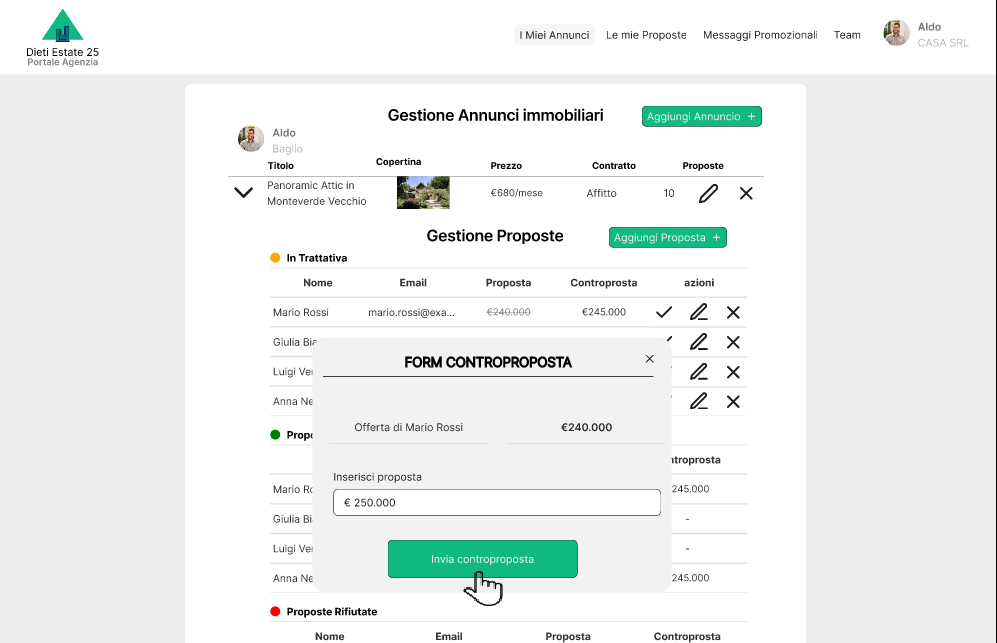
\includegraphics[width=0.7\textwidth]{Immagini/Mockup/controproposte/scenario principale/ClickInviaControproposta.png} \\
				Cockburn: step 6.A
			\end{tabular}
		};
		
		% Nodo per immagine 3 con didascalia sotto, posizionato sotto img2
		\node (img2) [below=of img1] {
			\begin{tabular}{c}
				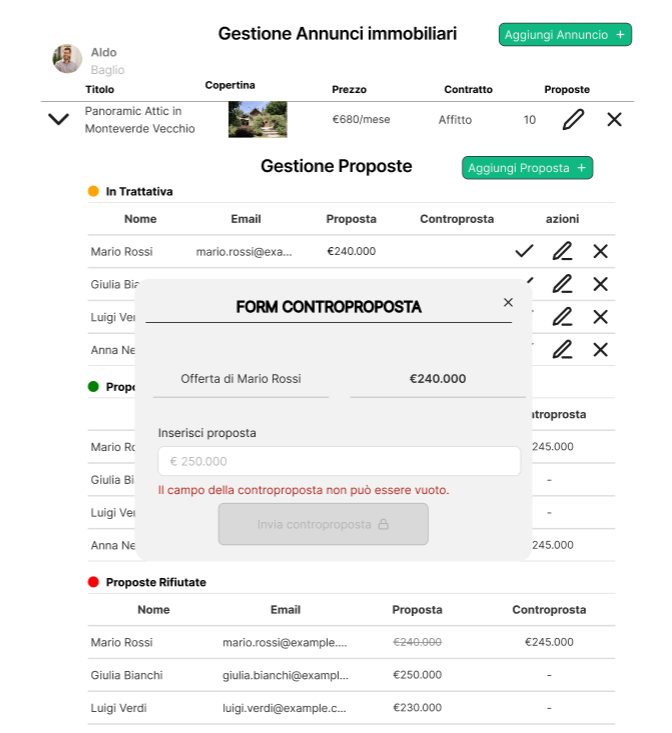
\includegraphics[width=0.7\textwidth]{Immagini/Mockup/controproposte/Extensions A/MessaggioDiErrore.png} \\
				Cockburn: step 7.A
			\end{tabular}
		};
		
		% Disegna le frecce
		\draw[->, thick] (img1) -- (img2);
		
	\end{tikzpicture}
	\caption{Mockup: Extension A della tabella di Cockburn del caso d'uso: Fare una controproposta a un'offerta.}
	\label{fig:tikz_flow}
\end{figure}

\newpage


